%!TEX root = ./template-skripsi.tex
%-------------------------------------------------------------------------------
%                            	BAB III
%               		    METODE PENELITIAN
%-------------------------------------------------------------------------------

\chapter{Metode Penelitian}

\section{Flow Penelitian}

\begin{figure}
  \centering{}
  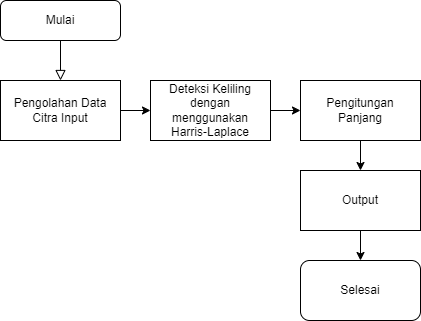
\includegraphics[width=0.45\textwidth]{gambar/Flowchart Penelitian.png}
  \caption{Diagram Penghitungan panjang ikan}
\end{figure}

\begin{figure}
  \centering{}
  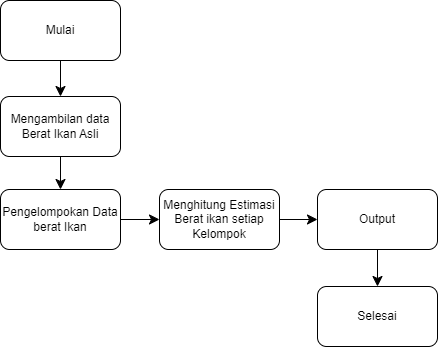
\includegraphics[width=0.45\textwidth]{gambar/Penghitungan Berat.png}
  \caption{Diagram Penghitungan berat ikan}
\end{figure}

\section{Deskripsi Sistem}

Dalam Penelitian yang akan dibuat adalah sebuah sistem yang dapat menghitung panjang serta berat rata-rata dari se-ekor ikan dengan menggunakan metode \emph{Harris-Corrner}.
Fokus dari penulis terhadap penelitian ini adalah untuk menghitung panjang serta berat rata-rata dari objek ikan. 
Citra yang digunakan oleh penulis diambil dari sebuah peternakan ikan, dimana citra tersebut akan penulis gunakan dalam pengujian sistem penghitungan panjang serta berat rata-rata ikan.

Bahasa yang penulis gunakan dalam perancangan sistem adalah Python 3. 
Tujuan penelitian adalah mendapatkan hasil perhitungan panjang dan berat ikan secara komputasi yang mana dihasilkan panjang dan berat ikan dari sebuah citra ikan. 

Tahapan yang akan diproses dalam penghitungan berat dan panjang ikan dengan menggunakan \emph{Harris-corner} adalah memasukan atau menginput citra ikan, lalu mendeteksi korner dari ikan menggunakan \emph{Harris-corner} dan menghitung panjang serta berat ikan mengunakan korner hasil dari \emph{Harris-corner}. 



